\section{Theorie}
\label{sec:theorie}

\subsection{Berechnung der Suszeptibilität}

In Anwesenheit von Materie ändert sich ein Magnetfeld $\vec{B} = \mu_0 \vec{H}$ um die Magnetisierung
\begin{equation*}
    \vec{M} = N \mu_0 \bar{\vec{\mu}} = \mu_0 \chi \vec{H} \,,
\end{equation*}
wobei $\bar{\vec{\mu}}$ das mittlere magnetische Moment und $\chi$ die Suszeptibilität darstellt.
Dabei ist $\chi$ keine Konstante, sondern eine von dem Magnetfeld $\vec{H}$ und der Temperatur $T$ abhängige Größe. \\

Je nach Bereich der Suszeptibilität werden unterschiedliche Arten von Magnetismus unterschieden.
Ist die Suszeptibilität kleiner null, wird von Diamagnetismus gesprochen.
Diese Form des Magnetismus beschreibt die Induktion zum äußeren Magnetfeld entgegengerichteter magnetische Momente. \\

Hier soll der Fokus aber stärker auf dem Paramagnetismus liegen.
Der Paramagnetismus stellt, entgegen zum Diamagnetismus, keine allgemeine Eigenschaft dar, er findet sich nur bei
Teilchen, die einen nicht verschwindenden Drehimpuls besitzen und entsteht durch die Orientierung der an den
Drehimpuls gekoppelten magnetischen Momente zum äußeren Feld. \\

Der Gesamtdrehimpuls setzt sich jedoch nicht nur aus dem Bahndrehimpuls zusammen, sondern besteht auch dem
Elektronen- bzw. Kernspin, dabei kann der Kernspin vernachlässigt werden.%Korrektur
Mit dem Gesamtspin $\vec{S}$ und dem Bahndrehimpuls $\vec{L}$ gilt für den Gesamtdrehimpuls
\begin{equation*}
    \vec{J} = \vec{L} + \vec{S} \,.
\end{equation*} \\

Die zu den Drehimpulsen gehörigen magnetischen Momente sind dabei durch

\begin{equation*}
    \vec{\mu_L} = -\dfrac{\mu_\text{B}}{\hbar} \vec{L}
    \label{eq:magmomL}
\end{equation*}
und
\begin{equation*}
    \vec{\mu_S} = - g_\text{S} \dfrac{\mu_\text{B}}{\hbar} \vec{S}
\end{equation*}
gegeben, wobei
\begin{equation*}
    \mu_\text{B} := \frac{\text{e}_0}{\text{m}_0} \hbar
\end{equation*}
das Bohrsche Magneton und $g_\text{S}$ das \textit{gyromagnetische Verhältnis des freien Elektrons}. \\

Werden nur die Beträge betrachtet, gilt
\begin{align}
    |\vec{L}| &= \sqrt{L(L + 1)} \hbar \,, \quad (L = \text{Bahndrehimpulsquantenzahl des Atoms}) 
    \label{eq:Labs} \\
    |\vec{S}| &= \sqrt{S(S + 1)} \hbar \quad (S = \text{Spinquantenzahl des Atoms})
    \label{eq:Sabs}
\end{align}
sowie
\begin{equation*}
    |\vec{J}| = \sqrt{J(J + 1)} \hbar \quad (J = \text{Gesamtdrehimpulsquantenzahl des Atoms}).
    \label{eq:Jabs}
\end{equation*} \\

Daraus folgt
\begin{equation}
    |\vec{\mu_\text{L}}| = \mu_\text{B} \sqrt{L(L + 1)}
    \label{eq:muLabs}
\end{equation}
und
\begin{equation}
    |\vec{\mu_\text{S}}| = \mu_\text{B} \sqrt{S(S + 1)} \,.
    \label{eq:muSabs}
\end{equation} \\

Aus \eqref{eq:muLabs} und \eqref{eq:muSabs} lässt sich nun das zum Gesamtdrehimpuls gehörende magnetische Moment
berechnen.
Es gilt
\begin{equation*}
    |\vec{\mu_\text{J}}| = |\vec{\mu_\text{S}}| \cos \alpha + |\vec{\mu_\text{L}}| \cos\beta \,,
\end{equation*}
wobei die Winkel $\alpha$ und $\beta$ wie in \autoref{fig:abb1} zu erkennen gewählt sind.

\begin{figure}[H]
    \centering
    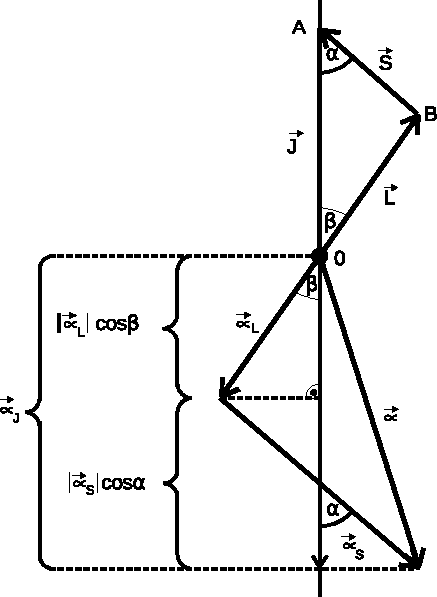
\includegraphics{figures/Abb_1.pdf}
    \caption{Vektordiagramm der magnetischen Momente $\,$ \cite{ap07}.}
    \label{fig:abb1}
\end{figure} 

Unter Verwendung des Cosinussatzes gilt
\begin{equation*}
    \cos\alpha = \dfrac{|\vec{J}|^2 - |\vec{L}|^2 + |\vec{S}|^2}{2|\vec{J}| |\vec{S}|}
\end{equation*}
und
\begin{equation*}
    \cos\beta = \dfrac{|\vec{J}|^2 - |\vec{L}|^2 + |\vec{S}|^2}{2|\vec{J}| |\vec{L}|} \,,
\end{equation*}
mit einigen Vereinfachung folgt dann
\begin{equation*}
    |\vec{\mu}_\text{J}| \approx \mu_\text{B} \sqrt{J(J + 1)} \dfrac{3 J (J + 1) + {S(S + 1) - L(L +1)}}{2J(J + 1)} \,.
\end{equation*} \\

Dabei ist 
\begin{equation}
    g_\text{J} := \dfrac{3 J(J + 1) + {S(S + 1 - L(L + 1))}}{2 J(J + 1)} \,,
    \label{eq:lande-faktor}
\end{equation}
der Landé-Faktor des Atoms. \\

Damit vereinfacht sich der Ausdruck zu 
\begin{equation*}
    |\vec{\mu}_\text{J}| \approx \mu_\text{B} g_\text{J} \sqrt{J(J + 1)} \,.
\end{equation*} \\

Unter Beachtung des quantenmechanischen Phänomens der Richtungsquantelung, das besagt, dass für die $\mu_{\text{J}_\text{Z}}$ nur ganzzahlige Vielfache von $\mu_\text{B}g_\text{J}$ möglich sind, folgt,
dass, relativ zur äußeren Feldrichtung, genau $2J + 1$ Einstellmöglichkeiten des magnetischen Moments mit einer potentiellen Energie von
\begin{equation*}
    E_\text{m} = - \vec{\mu}_\text{J} \cdot \vec{B} = \mu_{\text{J}_\text{Z}} B = \mu_\text{B} g_\text{J} m B
\end{equation*}
existieren. \\

Diese Aufspaltung der Energie in Unterniveaus wird als Zeeman-Effekt bezeichnet.
Mit der durch die Boltzmannverteilung gegebenen Besetzungshäufigkeit
\begin{equation*}
    Z(E,T) = \text{e}^{-\frac{E}{\text{k}T}}
\end{equation*}
und Summation über alle Einzelorientierung folgt nach einigen Rechenschritten
\begin{equation*}
    \chi = \dfrac{\mu_0 \mu^2_\text{B} g^2_J N J(J + 1)}{3 \text{k} T}
    \label{eq:susg_J}
\end{equation*}
für die paramagnetische Suszeptibilität. \\

\subsection{Berechnung der Suszeptibilität seltener Erden}

Um die theoretische Suszeptibilität seltener Erd-Verbindungen zu ermitteln, wird nach den Hundschen Regeln der Gesamtdrehimpuls bestimmt.
Die Hundschen Regeln lauten:

\begin{enumerate}
    \item Die Einzelspins $\vec{s}_i$ kombinieren zum nach dem Pauli-Prinzip maximal möglichen Gesamtspin $\vec{S} = \sum\vec{s}_i$
    \item Die Einzelbahndrehimpulse $\vec{l}_i$ setzen sich so zusammen, dass der bei Erfüllung des Pauli-Prinzips und Regel 1 maximale Drehimpuls $\vec{L} = \sum \vec{l}_i$ entsteht.
    \item Der Gesamtdrehimpuls ist $\vec{J} = \vec{L} - \vec{S}$, wenn die Schale weniger als und $\vec{J} = \vec{L} + \vec{S}$, wenn die Schale mehr als zur Hälfte gefüllt ist.
\end{enumerate}

\subsection{Suszeptibilitätsmessung über Brückenschaltungen}

Zur experimentellen Bestimmung der Suszeptibilität wird eine nach \autoref{fig:abb2} aufgebaute Brückenschaltung verwendet.

\begin{figure}
    \centering
    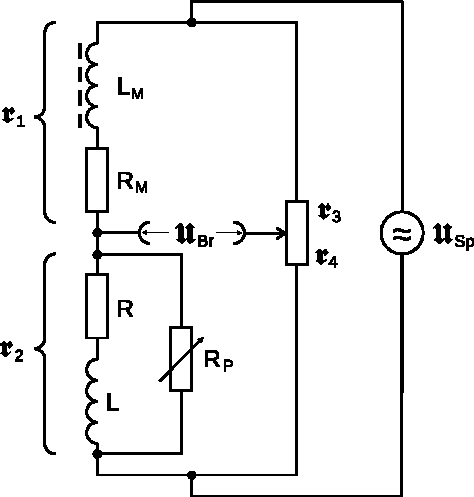
\includegraphics{figures/Abb_2.pdf}
    \caption{Brückenschaltung zur Suszeptibilitätsmessung$ \,$ \cite{ap07}.}
    \label{fig:abb2}
\end{figure}

Die totale Induktivität der mit Materie gefüllten Zylinderspule ist dabei gegeben durch
\begin{equation*}
    L_{M,\text{total}} = \mu \mu_0 \dfrac{n^2}{l} F \,,
    \label{eq:induspu}
\end{equation*}
mit der Windungszahl $n$, der Länge $l$ und dem Querschnitt $F$. \\

Ist die Spule nicht mit der Probe, sondern lediglich mit Luft gefüllt, kann der Faktor $\mu$ ignoriert werden, da $\mu_\text{Luft} \approx 1$, es gilt
\begin{equation*}
    L = \mu_0 \dfrac{n^2}{l} F \,.
\end{equation*} \\

Die Differenz $\Delta L$ zwischen der mit Luft und mit der Probe gefüllten Spule beträgt
\begin{equation*}
    \Delta L = \mu_0 \chi Q \dfrac{n^2}{l} \,,
\end{equation*}
wobei $Q$ der Probenquerschnitt ist. \\

Die komplexen Widerstände $Z_i$ sind dabei durch
\begin{align*}
    Z_1             &= R_\text{M} + i \omega L_\text{M} \, , \\
    \dfrac{1}{Z_2}  &= \dfrac{1}{R_\text{P}} + \dfrac{1}{R + i \omega L} \approx \dfrac{1}{ R + i \omega L} \, ,\\
    Z_3             &= R_3                                               \approx R_4 \, \text{und} \\
    Z_4             &= R_4                                               \approx R_3 
\end{align*}
gegeben. \\

Die Suszeptibilität lässt sich dabei auf zwei Arten bestimmen.
Über eine Änderung der Brückenspannung, oder durch eine Widerstandsänderung via Abgleichbedingung nach Einführen der Probe. \\

Nach einiger Rechnung ergibt sich für die Suszeptibilitätsmessung über Spannungsänderung der Ausdruck
\begin{equation*}
    \chi = \dfrac{U_\text{Br}}{U_\text{Sp}} \dfrac{4 l}{\omega \mu_0 n^2 Q} \sqrt{R^2 + \omega^2 \left(\mu_0 \dfrac{n^2}{l} F \right)^2} \,,
    \label{eq:spannsusamogus}
\end{equation*}
der sich in hochfrequenter Näherung zu
\begin{equation}
    \chi(\omega \rightarrow \infty) = 4 \dfrac{F}{Q} \dfrac{U_\text{Br}}{U_\text{Sp}}
    \label{eq:spannsussimp}
\end{equation}
vereinfacht, wobei $U_\text{Br}$ die Brücken- und $U_\text{Sp}$ die Speisespannung darstellen. \\

Über die Abgleichbedingung 
\begin{equation*}
    Z_1 R_4 = Z_2 R_3
\end{equation*}
folgt mit dem geänderten Abgleichwiderstand
\begin{equation*}
    R_3' = R_3 + \Delta R
\end{equation*}
die Suszeptibilität
\begin{equation}
    \chi = 2 \dfrac{\Delta R}{R_3} \dfrac{F}{Q} \,.
    \label{eq:widsus}
\end{equation}




